\documentclass[12pt, a4paper, oneside]{ctexart}
\usepackage{amsmath, amsthm, amssymb, bm, color, framed, graphicx, hyperref, mathrsfs, mathtools, enumerate, tikz}
\usepackage{graphicx}
\usepackage{float}
\usepackage{subfig}

\usetikzlibrary{patterns}

\title{\textbf{Homework 4}}
\author{萃英学院\qquad 2022级\qquad 王一鑫}
\date{\today}
\linespread{1.5}
\newcounter{problemname}
\newenvironment{problem}{\begin{framed}\stepcounter{problemname}\par\noindent\textsc{Problem \arabic{problemname}. }}{\end{framed}\par}
\newenvironment{solution}{%
	\par\noindent\textsc{Solution. }\ignorespaces
}{%
	\hfill$\qed$\par
}
\newenvironment{note}{\par\noindent\textsc{Note of Problem \arabic{problemname}. }}{\\\par}

\begin{document}
	
	\maketitle
	
	\begin{problem}
		(Exercise 3.7)

        Find the fundamental sets of cycles and cutsets of the graph in Fig\ref{fig:3.7} associated with the spanning tree shown.
        \begin{figure}[H]
			\small
			\centering
			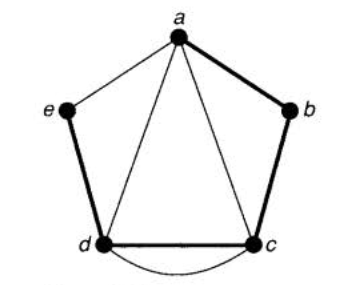
\includegraphics[width=0.5\columnwidth]{figure/fig1.png}
			\caption{Figure For Problem 1}
			\label{fig:3.7}
		\end{figure}


	\end{problem}
	
	\begin{solution}
		
        \begin{enumerate}
            \item \textbf{Cycles}: By definition, we can find $abcdea$, $abcda$, $abca$
            $cdc$.
            \item \textbf{Cutsets}: \{$ab$, $ae$, $ad$, $ac$\}; \{$bc$, $ae$, $ad$, $ac$\};
            \{$cd$, $ae$, $ad$, $cd$\}; \{$ed$, $ae$, $ad$\}.
        \end{enumerate}
		
	\end{solution}
		

		
	
	\begin{problem}
		(Exercise 3.10)

        If \( G \) is a connected graph, a \textbf{centre} of \( G \) is a vertex \( v \) 
        with the property that the maximum of the distances between \( v \) 
        and the other vertices of \( G \) is as small as possible. 
        By successively removing all the end-vertices, 
        prove that every tree has either one centre or two adjacent centres. 
        Give an example of a tree of each type with seven vertices.


	\end{problem}
	
	\begin{solution}
		
	We will follow the hint by removing all the end-vertices. Denote $M(v) = \max\{\text{d}(v,w)| w\in V(G)\}$.
    Notive that the maximum distance \( M(v) \) 
    from a given vertex \( v \) to any other vertex \( w \) occurs only 
    when \( w \) is a end-vertex.

    First, let \( G \) be a tree with \( n \) vertices (\( n \geq 2 \)).
    Then $G$ must have at least two end-vertices. Delete all end-vertices from \( G \), then the resulting graph \( G' \) is still a tree.

    After removing end-vertices, $E(v)$ in  $G'$ is just one less than $E(v)$ in  $G'$.
    Again, delete end-vertices from \( G' \) so that the resulting \( G'' \) is still a tree with the same centers.

    Note that all vertices that \( G \) had as centers will still remain centers 
    in \( G' \rightarrow G'' \rightarrow G''' \dots \).
    Continue this process until the remaining tree has either one vertex or one edge.

    So at the end, if one vertex is there this implies tree \( G \) has one center.
    If one edge is there then tree \( G \) has two centers which are adjacent.

    One example with seven vertices are shown as Fig\ref{fig:7V}.
    \begin{figure}[H]
		\small
		\centering
		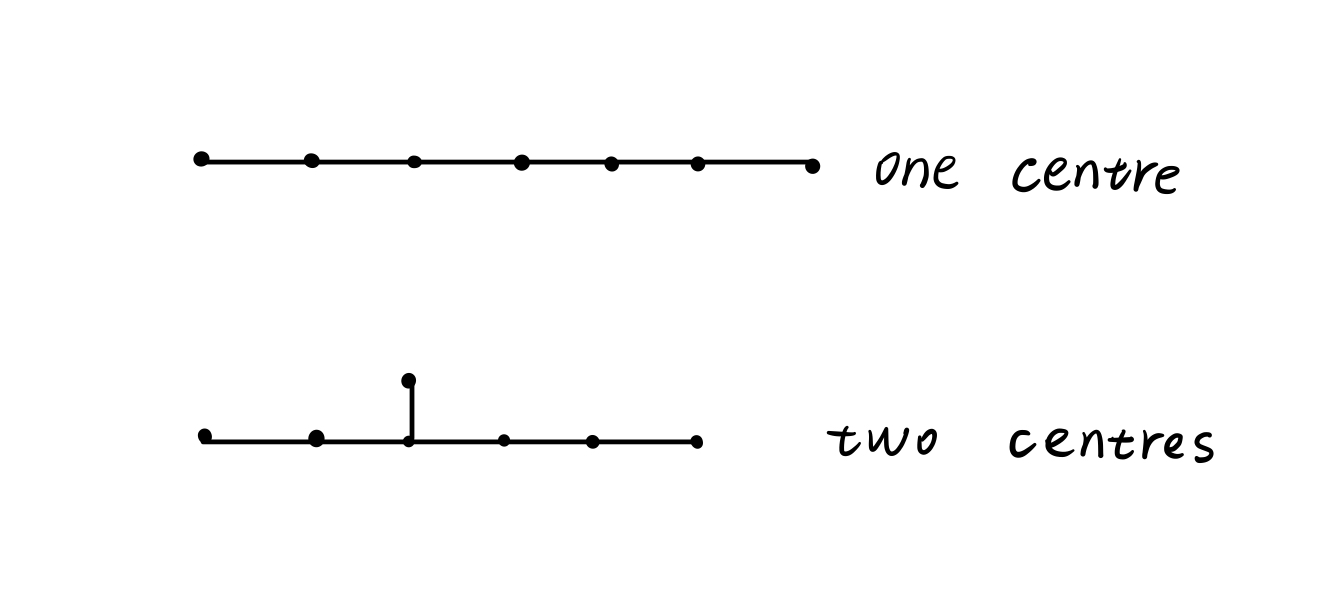
\includegraphics[width=0.75\columnwidth]{figure/fig2.jpg}
		\caption{Example}
		\label{fig:7V}
	\end{figure}


		
	\end{solution}
	
	\begin{problem}
        (Exercise 3.11)

		
        Let \( T_1 \) and \( T_2 \) be spanning trees of a connected graph \( G \).
        \begin{enumerate}[(i)]
            \item If \( e \) is any edge of \( T_1 \), show that there exists an edge \( f \) of \( T_2 \) 
            such that the graph \( (T_1 - \{e\}) \cup \{f\} \) 
            (obtained from \( T_1 \) on replacing \( e \) by \( f \)) is also a spanning tree.

            \item Deduce that \( T_1 \) can be `transformed' into \( T_2 \) by replacing the edges 
            of \( T_1 \) one at a time by edges of \( T_2 \) in such a way that a spanning tree is obtained 
            at each stage. (This result will be needed in Chapter 7.)

        \end{enumerate}

	\end{problem}
	
	\begin{solution}
        \begin{enumerate}[(i)]
            \item Let $e \in E(T_1)$. Removing  $e$ from  $T_1$ disconnects it into two components, $A$ and $B$.
            Since  $T_2$ is a spanning tree, it contains a unique edge $f$ connecting $A$ and $B$.
            Adding $f$ to $T_1 - \{e\}$ reconnects $A$ and $B$
            resulting in a spanning tree $(T_1 - {e}) \cup {f}$. 
            \item  Let $k = |E(T_1) \setminus E(T_2)|$. If $k = 0$, then $T_1 = T_2$. Otherwise, 
            choose $e \in E(T_1) \setminus E(T_2)$. 
            By (i), replace $e$ with some $f \in E(T_2)$ to get a new spanning tree $T_1'$ with 
            $|E(T_1') \setminus E(T_2)| = k - 1$. 
            Repeat this process inductively until all edges of $T_1$ are replaced by edges of $T_2$,
            maintaining a spanning tree at each step.
        \end{enumerate}
		   
		
	\end{solution}
	
	
	
	\begin{problem}
		(Exercise 3.12)

        Verify directly that there are exactly 125 labelled trees on five vertices.

		
	\end{problem}
	
	\begin{solution}

		For unlabelled trees on five vertices, there are three cases sohwn in Fig\ref{fig:3C}.
        \begin{figure}[H]
            \small
            \centering
            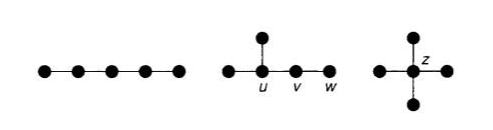
\includegraphics[width=0.75\columnwidth]{figure/fig3.png}
            \caption{unlabelled Trees}
            \label{fig:3C}
        \end{figure}
		For the firs tree, there are $5!/2 = 60$ labelled trees. For the second one, there are $5\times 4\times 3$ labelled trees,
        depending on the different choices of $u$, $v$ and $w$. For the last one, there are $5$ labelled trees depending on $z$.

        Therefore, there are exactly $125$ labelled trees on five vertices.
		
	\end{solution}


	\begin{problem}
		
    Show that, for each value of \( n \), the graph associated with the alcohol
    \( C_n H_{2n+1} OH \) is a tree (the oxygen vertex has degree 2). 
    Draw the tree corresponding to the molecule \( C_2 H_5 OH \).

		% \begin{figure}[h]
	
		% 	\begin{minipage}{0.32\linewidth}
		% 		\vspace{3pt}
				
		% 		\centerline{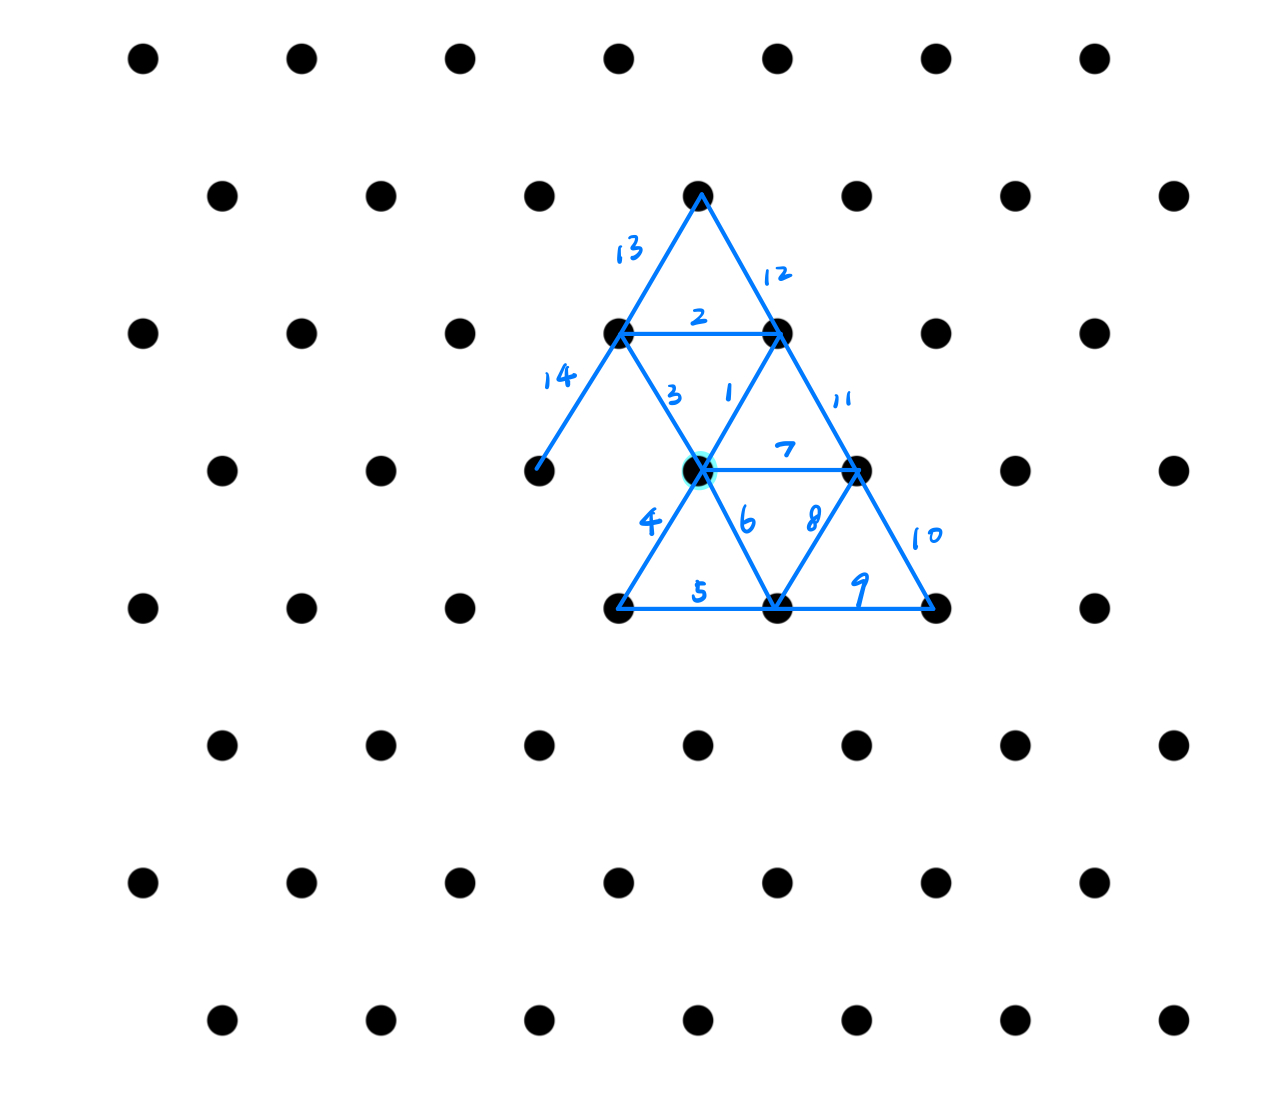
\includegraphics[width=\textwidth]{figure/fig6.png}}
			
		% 		\centerline{Step 1}
		% 	\end{minipage}
		% 	\begin{minipage}{0.32\linewidth}
		% 		\vspace{3pt}
		% 		\centerline{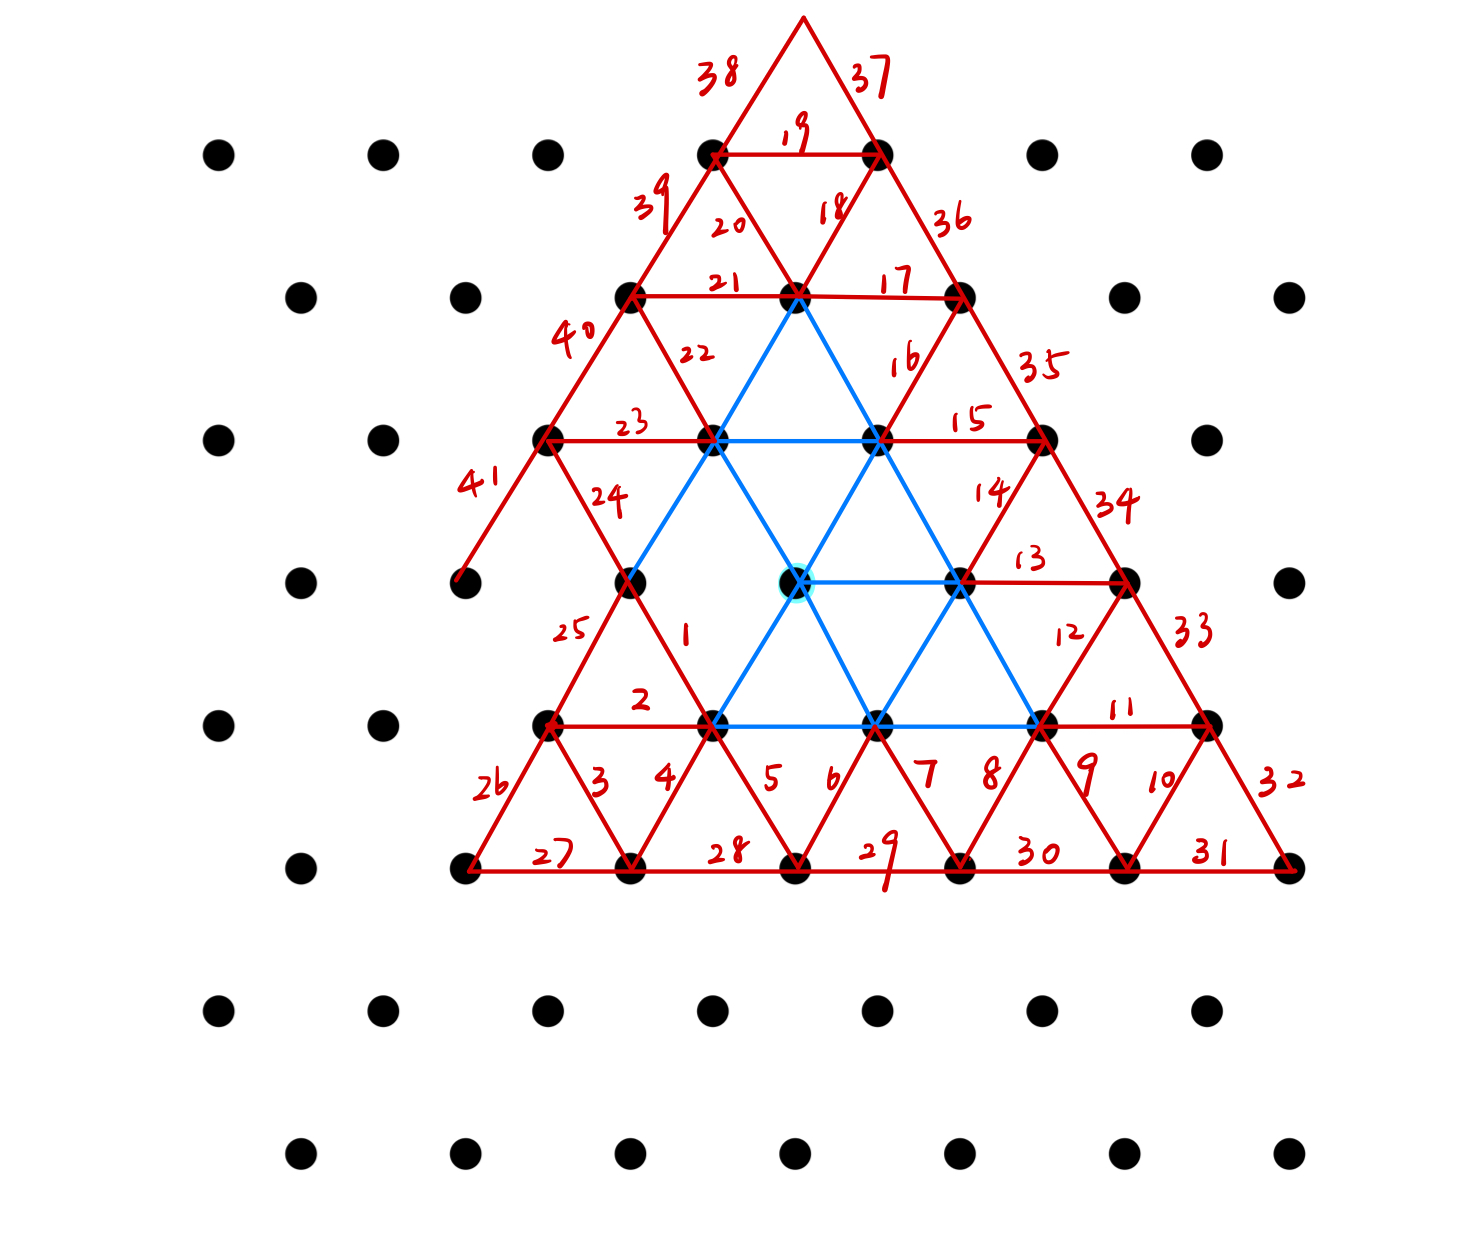
\includegraphics[width=\textwidth]{figure/fig7.png}}
			 
		% 		\centerline{Step 2}
		% 	\end{minipage}
		% 	\begin{minipage}{0.32\linewidth}
		% 		\vspace{3pt}
		% 		\centerline{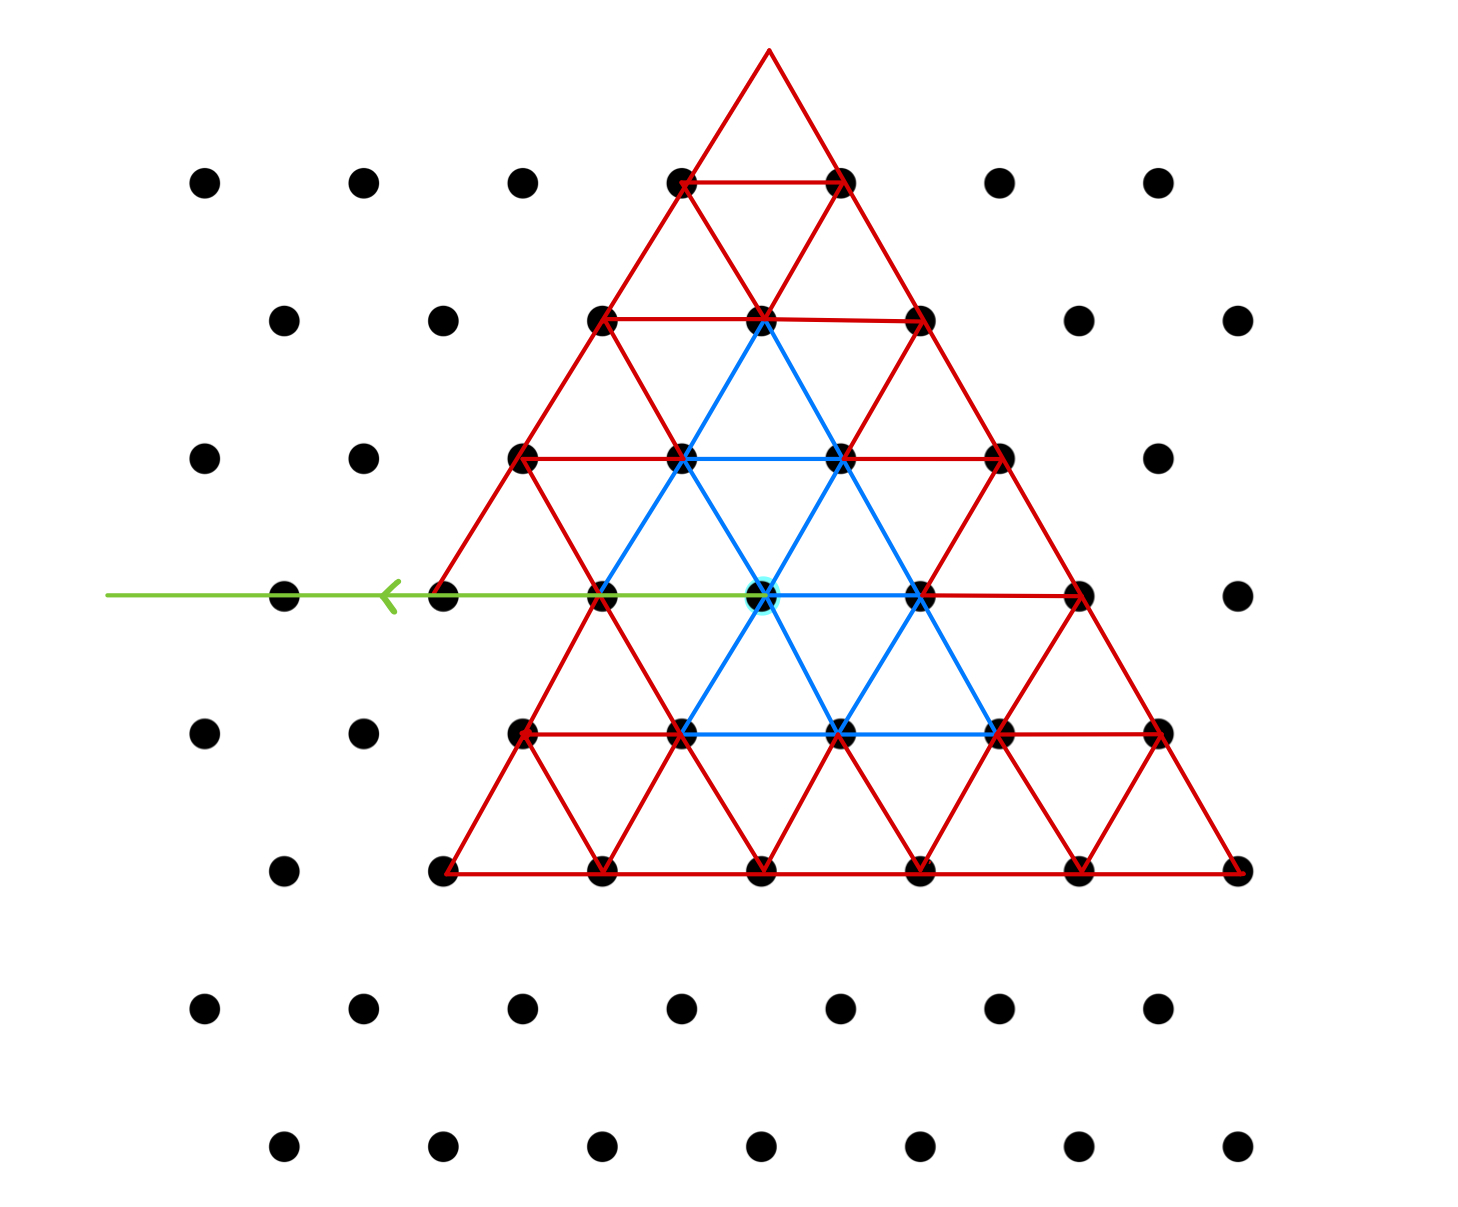
\includegraphics[width=\textwidth]{figure/fig8.png}}
			 
		% 		\centerline{Step 3}
		% 	\end{minipage}
		% 	\caption{Construction of Euler trail}
		% 	\label{fig:Construction}
		% \end{figure}
		
    \end{problem}

	\begin{solution}
        
		The graph is a connected graph. We can calculate the number of vertices and edges:
    \begin{enumerate}
        \item \textbf{Vertices}: $n + (2n + 1) + 1 + 1 = 3n + 3$.
        \item \textbf{Edges}: $\dfrac{1}{2}(4n + (2n + 1) + 2 + 1) = 3n + 2$.
    \end{enumerate}
    This is directly from the property of \( C_n H_{2n+1} OH \), and is therefore a tree, by Theorem 3.1(iii).
    The tree corresponding is shown in Fig \ref{fig:Al}.
    
    \begin{figure}[H]
        \small
        \centering
        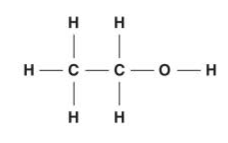
\includegraphics[width=0.5\columnwidth]{figure/alcohol.png}
        \caption{Tree of Alcohol}
        \label{fig:Al}
    \end{figure}
    \end{solution}
		
    
	\begin{problem}
		(Exercise 3.16)
         
        In the first proof of Cayley's theorem, find the labelled tree that 
        corresponds to the sequence \( (7, 6, 5, 4, 3, 2, 1) \).


    \end{problem}

	\begin{solution}
		
		Follow the construction in the proof of Cayley's theorem, we find the desired labelled tree in Fig \ref{fig:lt}

		\begin{figure}[H]
			\small
			\centering
			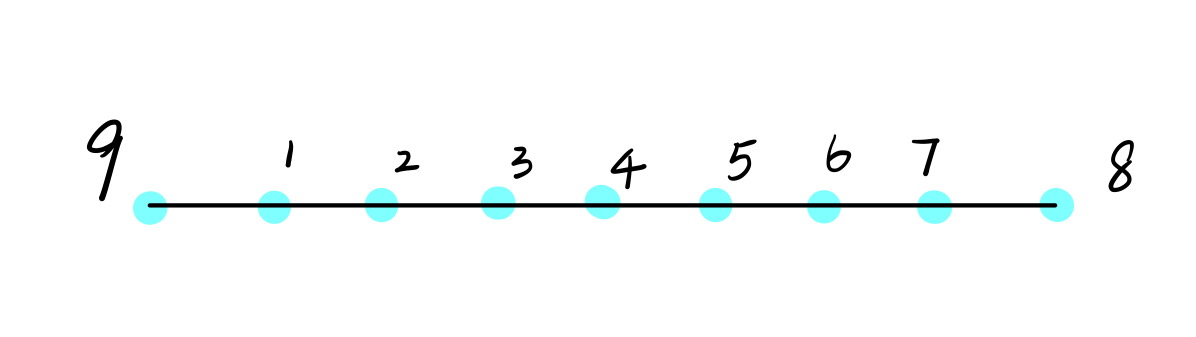
\includegraphics[width=0.5\columnwidth]{figure/fig4.jpg}
			\caption{Labelled Tree}
			\label{fig:lt}
		\end{figure}
		
	\end{solution}


	\begin{problem}
		
        Show that every tree with maximum degree \( k \) has at least \( k \) leaves.

	\end{problem}

	\begin{solution}

    The case \( k = 1 \) is trivial. 
    Assume that \( k \geq 2 \). Let \( u \) be a vertex of degree \( k \) - So \( u \) is not a leaf.

    We have 
    \[
    \sum_{v \in V} \text{deg} \, v = 2|E|
    \]
    in every graph. Also,
    \[
    |E| = |V| - 1
    \]
    in every tree. Thus
    \[
    \sum_{v \in V} \text{deg} \, v = 2|V| - 2
    \]

    Define \( L \) to be the set of leaves of the graph. 
    The degree of every non-leaf vertex is at least 2, so it follows 
    \[
    \sum_{v \in V} \text{deg} \, v = \text{deg} \, u + \sum_{v \in L} \text{deg} \, v + \sum_{v \in V \setminus (L \cup \{u\})} \text{deg} \, v \geq k + |L| + 2(|V| - |L| - 1)
    \]
    Thus
    \[
    2|V| - 2 \geq k + 2|V| - |L| - 2
    \]
    and it follows that \( |L| \geq k \).


	\end{solution}

	
\end{document}


